
\chapter{Functional/Geometric Bias In Neural Language Models}
\chaptersource{Simon Dobnik, Mehdi Ghanimifard and John Kelleher.}{Exploring the functional and geometric bias of spatial relations using neural language models,}{In Proceedings of the First International Workshop on Spatial Language Understanding, pp. 1-11. 2018.}

\paragraph{Abstract}
  The challenge for computational models of spatial descriptions for
  situated dialogue systems is the integration of information from
  different modalities. The semantics of spatial descriptions are
  grounded in at least two sources of information: (i) a
  geometric representation of space and (ii) the functional interaction
  of related objects that. We
  train several neural language models on descriptions of scenes from
  a dataset of image captions and examine
  whether the functional %
  or geometric %
  bias of spatial descriptions reported in the literature is reflected
  in the estimated perplexity of these models. The results of these experiments have implications for the creation of models of spatial lexical semantics for human-robot dialogue systems. Furthermore, they also provide an insight into the kinds of the semantic knowledge captured by neural
  language models trained on spatial descriptions, which has implications for image captioning systems.



\section{Introduction}\label{splu2018:sec:spatial-descriptions}

Spatial language understanding is fundamental requirement for human-robot interaction through dialogue. A natural task for a human to request a robot to fulfil is to retrieve or replace an object for them. Consequently, a particularly frequent form of spatial description within human-robot interaction is a \emph{locative expression}. A locative expression is a noun phrase that describes the location of one object (the \emph{target object}) relative to another object (the \emph{landmark}). The relative location of the target object is specified through a %
prepositional phrase:
\begin{center}
Bring~me~$\underbrace{\underbrace{the~big~red~book}_{Target}~\underbrace{on~\underbrace{the~table}_{Landmark}}_{\substack{Prepositional\\Phrase}}}_{Locative~Expression}$.
\end{center}
\noindent In order to understand these forms of spatial descriptions a robot must be equipped with computational models of the spatial semantics of prepositions that enable them to ground the semantics of the locative expression relative to the context of the situated dialogue.

A natural approach to developing these computational models is to define them in terms of scene \emph{geometry}. And, indeed, there is a tradition of research that follows this path, see for example \cite{logan/sadler:1996,KelleherCostello:2005,KelleherCostello:2009}. However, there is also a body of experimental and computational research that has highlighted that the semantics of spatial descriptions are dependent on several sources of information beyond scene geometry, including \emph{functional semantics} (which encompasses a range of factors such as world knowledge about the typical interactions between objects, and object affordances) \cite{Coventry:2004aa}. We can illustrate this distinction between geometric and functionally
defined semantics using a number of examples. To illustrate a geometric semantics: assuming a spatial meaning, anything
can be described as \emph{to left of} anything else so long the spatial configuration of the two objects is geometrically correct.
However, as \cite{CoventryEtAl:2001} has shown the spatial description \emph{the umbrella is over the man} is sensitive to the
 protective affordances of the umbrella to stop rain, and is appropriate in contexts where, the umbrella is not in a
geometrically prototypical position above the man, so long as the umbrella is protecting the man from the rain.

A further complication with regard to modelling the semantics of spatial descriptions is that experimental results indicate that the contribution of geometrical and
functional factors is not the same for every spatial relation \citep{Garrod:1999fk,CoventryEtAl:2001}.  This experimental work shows that there is
an interplay between function and geometry in the definition of spatial semantics
and therefore the spatial meaning of given spatial relation is neither fully functional nor fully geometric. Rather, spatial terms can be ordered on a spectrum
based on the sensitivity of their semantics to geometric or functional factors.

Given the distinction between geometric and functional
factors in shaping spatial semantics, a useful analysis that
would inform the design and creation of computational models of spatial
semantics is \emph{to identify the particular semantic bias
(geometric/functional) that each spatial term evinces}. However, such an analysis is difficult. Native speakers do not have strong intuitions about the bias of
prepositions and such bias had to be established experimentally
\cite{CoventryEtAl:2001,Garrod:1999fk} or through linguistic analysis
\cite[p.55]{herskovits1986language}.\footnote{The discussion of Herskovits
  focuses on interaction of objects conceptualised as geometric
  shapes, for example \emph{on:} contiguity with line or surface. The
  fact that the interacting objects can be conceptualised as different
  geometric shapes points and therefore related by a particular
  prepositions points to their functional nature as discussed here.}
Reviewing the literature on this experimental and analytic work reveals
that prepositions such as \emph{in}, \emph{on}, \emph{at}, \emph{over}, \emph{under}
have been identified as being functionally biased, whereas \emph{above}, \emph{below}, \emph{left of} and \emph{right of} are geometrically biased. Other spatial
relations may be somewhere in between. In this paper we will use these relations as ground-truth pointers against which our methods will be evaluated. If the method is successful, then we are able to make predictions about those relations that have not been verified for their bias experimentally. Knowing the bias of a spatial relation is useful both theoretically and practically. Theoretically, it informs us about the complexity of grounded semantics of spatial relations. In particular, it engages with the ``what'' and ``where'' debate where it has been argued that spatial relations are not only spatial (i.e. geometric) \cite{Landau:1993aa,Coventry:2004aa,Landau:2016aa}. Practically, the procedure to estimate the bias is useful for natural language generation systems, for example in situated robotic applications that cannot be trained end-to-end. Given that a particular pair of objects can be described geometrically with several spatial relations, the knowledge of functional bias may be used as a filter, prioritising those relations that are more likely for a particular pair of objects, thereby incorporating functional knowledge. This approach to generation of spatial descriptions is therefore similar to the approach that introduces a cognitive load based hierarchy of spatial relations \cite{Kelleher:2006} or a classification-based approach that combines geometric (related to the bounding box), textual (word2vec embeddings) and visual features (final layer of a convolutional network) \cite{Ramisa:2015aa}. The functional geometric bias of spatial relations could also be used to inform semantic parsing, for example in prepositional phrase attachment resolution \cite{Christie:2016aa,Delecraz:2017aa}.

Previous work has investigated metrics of the semantic bias of spatial prepositions, see \cite{Dobnik:2013aa,Dobnik:2014ab}. \citep{Dobnik:2013aa} uses (i) normalised entropy of target-landmark pairs to estimate variation of targets and landmarks per relation and (ii) log likelihood ratio
to predict the strength of association of target-landmark pairs with a
spatial relation and presents ranked lists of relations by the degree of argument variation or
strength of the association respectively. The approach hypothesises that
functionally biased relations are more selective in the kind of
targets and landmarks they co-occur with. The reasoning behind this is that geometrically it is possible to relate a wider range of objects than in the case where additional functional constrains between objects are also applied. \cite{Dobnik:2014ab}
generalises over landmarks and targets in WordNet hierarchy and
estimates the generality of the types of landmark. Again, the work
hypothesises that functional relations are more restricted in their
choice of target and landmark objects and therefore are generally more
specific in terms of the WordNet hierarchy. Both papers present
results compatible with the hypotheses where the functional or
geometric nature of prepositions is predicted in line with the
experimental studies \cite{Garrod:1999fk,CoventryEtAl:2001}.

Sensitive to the fact that relations such as \emph{in} and \emph{on} not only have spatial usage
but also usages that may be considered metaphoric \cite{Steen:2010aa}, both \cite{Dobnik:2013aa} and \cite{Dobnik:2014ab} were based on an analysis of a corpus of image captions. The idea being that descriptions of images are
more likely to contain spatial descriptions grounded in the image. %
For similar reasons, we also employ a corpus %
of image descriptions (larger than in the previous work).








This paper adopts a similar research hypothesis to
\cite{Dobnik:2014ab,Dobnik:2013aa}, namely that: it is possible to
distinguish between functionally biased and geometrically biased spatial relations by examining the
diversity of the contexts in which they occur. Defining the concept of context in terms
of the \emph{target} and \emph{landmark} object pairs that a relation occurs within, the rationale of this
hypothesis is that: geometrically biased relations are more likely to be observed in a more diverse set of
contexts, compared to functionally biased relations, because the use of a geometrically biased relation
 only presupposes the appropriate geometric configuration whereas the use of a functionally biased
 relation is also constrained by object affordances or typical interactions.


 However, the work presented in this paper provides a more general
 analytical technique based on a neural language model
 \cite{bengio2003neural,mikolov2010recurrent} which is applied to a
 larger dataset of spatial descriptions. 
 We use neural language models as the basic tool for our analysis because
 they are already commonly used to learn the syntax and semantics of
 words in an unsupervised way.
 The contribution of
 this paper in relation to (i) the previous analyses of geometric and
 functional aspects of spatial relations is that it examines whether
 similar predictions can be made using these more general tools of
 representing meaning of words and phrases; the contribution to (ii)
 deep learning of language and vision is that it examines to what
 extent highly specific world-knowledge can be extracted from a
 neural language model. The paper proceeds as follows: in
 Section~\ref{splu2018:sec:dataset} we describe the datasets and their
 processing, in Section~\ref{splu2018:sec:lm-perplexity} we describe the basics
 behind language models and the notion of perplexity, in
 Section~\ref{splu2018:sec:plain-perplexity} and \ref{splu2018:sec:swapability} we
 present and discuss our results. We conclude in
 Section~\ref{splu2018:sec:discussion}.

 The code that was used to produce the datasets and results discussed
 in this paper can be found at: \\
 \url{https://github.com/GU-CLASP/functional-geometric-lm}.
 






\section{Datasets}\label{splu2018:sec:dataset}

The Amsterdam Metaphor Corpus \cite{Steen:2010aa} which is based on a subsection of a BNC reveals that the spatial sense of prepositions are very rare in genres such as news, fiction and academic texts. For example, \emph{below} only has two instances that are not labelled as a metaphor and more than 60\% of fragments with \emph{in}, \emph{on}, and \emph{over} are not used in their spatial sense. %
For this reason \citet{Dobnik:2013aa} use %
two image description corpora (IAPR TC-12 \cite{Grubinger:2006uq} and
Flickr8k \cite{Rashtchian:2010kx}) where spatial uses of prepositions are common.  They apply a dependency parser and a set of post-processing rules to extract spatial relations, target and landmark object triplets. %
The size of this extracted dataset is 96,749 instances %
and is relatively small for training a neural language model. %
\cite{Kordjamshidi:2017ab} released CLEF 2017 multimodal spatial role labelling dataset (mSpRL) which is a human annotated subset of the IAPR TC-12 Benchmark corpus for spatial relations, targets and landmarks \cite{Kordjamshidi:2011aa} containing 613 text files and 1,213 sentences. While this dataset could not be used to train a language model directly, a spatial role labelling classifier could be trained on it to identify spatial relations and arguments which would then be used to produce a bootstrapped dataset for training a neural language model.


Recently, Visual Genome \cite{Krishna:2016aa} has been released which
is a crowd-source annotated corpus of 108K images which also includes
annotations of \emph{relationships} between (previously annotated)
bounding boxes. Relationships are predicates that relate objects which
include spatial relations (2404639, ``cup on table''), verbs (2367163,
``girl holding on to bear'') as well as combinations of verbs and
spatial relations (2317920, ``woman standing on snow'') and others.
We use this dataset in the work reported here. Its advantage is that
it contains a large number of annotated relationships but the
disadvantage is that these are collected in a crowd-sourced setting
and are therefore sometimes noisy but we assume these are still of better quality
than those from a bootstrapped machine annotated dataset.

To extract spatial relations from the annotated relationships, we
created a dictionary of their syntactic forms based on the lists
of English spatial relations in \citet{Landau:1996aa} and %
\citet{herskovits1986language}. %
For the training data we preserve all items annotated as relationships as single tokens (``jumping\_over'')
and we simplify some of the composite spatial relations based on our dictionary, e.g. ``left of''
and ``to the left of'' become ``left'' %
to increase the frequency of instances. This choice could have affected our results if done without careful consideration. While compound variants of spatial relations have slightly different meanings, we only collapsed those relations for which we assumed this would not affect their geometric or functional bias. Furthermore, \citet{Dobnik:2013aa} show that compound relations cluster with their non-compound variants using normalised entropy of target-landmark pairs as a metric. Finally, some variation was due to the shorthand notation used by the annotators, e.g. ``to left of''.  The reason behind keeping all relation(ships) in the training set is to train the language model on as many targets and landmarks as possible and to learn paradigmatic relations between them. We normalise
all words to lowercase and remove the duplicate descriptions per image
(created by different annotators). We also check for and remove instances %
where a spatial relation is used as an object, e.g.
``chair on left''.
We remove instances where
one of the words has fewer than 100 occurrences in the whole dataset which reduces
the dataset size by 10\%.
We add start and end tokens to the triplets ($\langle s \rangle\ target\ relation\ landmark\ \langle /s \rangle$) as required for training and testing a language model.
The dataset is shuffled and split into 10 folds that are later used in cross-validation.
In the evaluation, we take 20 samples per spatial relation from the held out data of those relations that are members of the dictionary created previously. This way the average perplexity is always calculated on the same number of samples per each relation.\footnote{The reason we use 20 sample is that this is also the size of the 10\% test folds in the down-sampled dataset described later. In selecting 20 items for the test-set we also ensure that it contains the vocabulary in the down-sampled training folds.}








\section{Language model and perplexity}\label{splu2018:sec:lm-perplexity}

\subsection{Language model}\label{splu2018:sec:lm-description}


Probabilistic language models capture the sequential properties of language or paradigmatic relations between sequences of words. Using the chain rules of probabilities they estimate the likelihood of a sequence of words: %
\begin{equation}\label{splu2018:eq:lm}
P(w_{1:T}) = \sum_{t=1}^{T}{P(w_{t+1} | w_{1:t})}
\end{equation}
\noindent Neural language models estimate %
probabilities by optimising parameters of a function represented in a neural architecture
\cite{bengio2003neural}:
\begin{equation}\label{splu2018:eq:nnlm}
{\hat{P}(w_{t+1}| w_{1:t} = v_{k_{1:t}})} = f(v_{t-1};\Theta) = \hat{y}_{t}
\end{equation}
\noindent where $\Theta$ represents parameters of the model, $f$ being the composition of
functions within the neural network architecture, and $v_{k_{1:t}}$ the words up to time $t$ in the sequence. The output of the function is $\hat{y}_{t} \in R^{n}$, a vector of %
probabilities, with each dimension representing the probability of a word in the vocabulary.
The loss of a recurrent language model is the average surprisal for each batch of data \cite{graves2013speech,mikolov2010recurrent}:
\begin{equation}\label{splu2018:eq:rnnloss}
loss(S) = -\sum_{s \in S} \sum_{t = 0}^{|s|} \frac{\text{log}(\hat{y}_{t}(v_{k_{t+1}}))}{|S| \times |s|}
\end{equation}
\noindent Note that our architecture is deliberately simple as we apply it in an experimental setting with constrained descriptions\footnote{For more details on the architecture see Section~\ref{splu2018:sec:lm}  in the supplementary material, in particular Figure~\ref{splu2018:fig:lm-diagram} and Equation~\ref{splu2018:eq:lm-parameters}.}.
We use a Keras implementation \cite{chollet2015keras}, and fit the model parameters with Adam \cite{kingma2014adam} 
with a batch size of 32 and iterations of 20 epochs. On each iteration the language model is optimised on the loss which is related to perplexity as described in the following section.




\subsection{Perplexity}

Instead of calculating the averages of
likelihoods from Equation~\ref{splu2018:eq:lm}, which might get very low on long sequences of text, we use perplexity which is an exponential measure for average negative log
likelihoods of the model. This solves the representation problem with
floating points and large samples of data.
\begin{equation}\label{splu2018:eq:perplexity}
  Perplexity(S, P) = 2^{E_S [ -log_2(P(w_{1:T})) ]} %
\end{equation}
\noindent where $w_{1:T}$ is an instance in a sample collection $S$. Perplexity is often used for evaluating language models on test sets. Since
language models are optimised for low perplexities\footnote{Equation~\ref{splu2018:eq:perplexity} is related to Equation~\ref{splu2018:eq:rnnloss} as perplexity is $2^{\textrm{Loss}}$ given a neural model as the likelihood model.}, %
the perplexity of a trained
model can be used as a measure of fit of the model with the samples.


\section{Varying targets and landmarks}\label{splu2018:sec:plain-perplexity}



\subsection{Hypotheses}


As a language model encodes semantic relations between words in a
sequence we therefore expect that the distinction between functional
and geometric spatial relations will also be captured by it.  As
functionally biased spatial relations are used in different
situational contexts than geometrically biased spatial relations, we
expect that a language model will capture this bias in different
distributions of target and landmark objects in the forms of the
perplexity of phrases. Our weak hypothesis is that the perplexity of phrases on the test set reflects the
functional-geometric bias of a spatial relation (Hypothesis 1). We take the assumption that functionally-biased
relations are more selective in terms of their target and landmark
choice (Section~\ref{splu2018:sec:spatial-descriptions}) and consequently sequences such as \texttt{$<$s$>$ target
  relation landmark $<$/s$>$} with functional relations have a higher predictability in the
dataset resulting in a lower perplexity in the language model
(Hypothesis 2). Related to this hypothesis, there is a stronger hypothesis that target and landmark are predictable with a given functional spatial relation (Hypothesis 3).








\subsection{Method}\label{splu2018:sec:plain-perplexity-method}

We train two language models as described in
Section~\ref{splu2018:sec:lm-description}. For training and evaluation 10-fold cross-validation is used and average results are reported. %
We ensure that the evaluation sets
contain no vocabulary not seen during the training. The language model 1
(LM1) is trained on unrestricted frequencies of instances. In training the language model 2 (LM2) we
down-sample relations so that they are represented with equal
frequencies. %
The dataset to train LM2 contains 200
instances of each possible relations %
while the evaluation set contains 20 instances for each spatial relation. Note that using this method
some targeted spatial relations might disappear from the evaluation
set as their frequency in the held-out data is too low. In addition to
the requirement that the evaluation set contains no
out-of-vocabulary items, the target and landmarks are included without restriction on their frequency, as they occur with these spatial relations.




\subsection{Results}



\begin{figure}[ht]
  \begin{center}
      \begin{minipage}{0.5\linewidth}
      	\centering
      	\hspace*{-1.2em}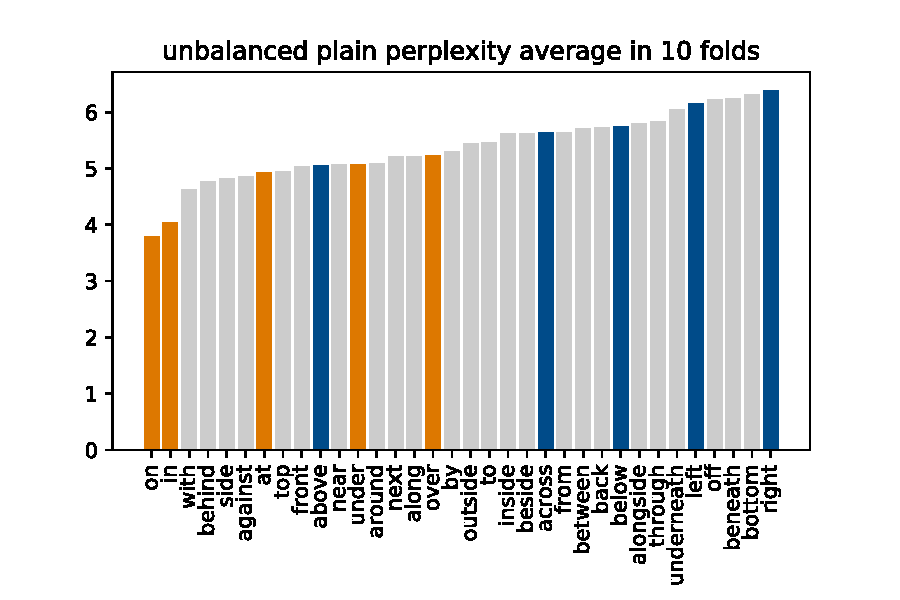
\includegraphics[width=1.12\linewidth]{studies/splu2018/figures/o_pp_cv-avg.pdf}\\
	  	(a) test-set 
    \end{minipage}%
	\begin{minipage}{0.5\linewidth}
		\centering
		\hspace*{-1.em}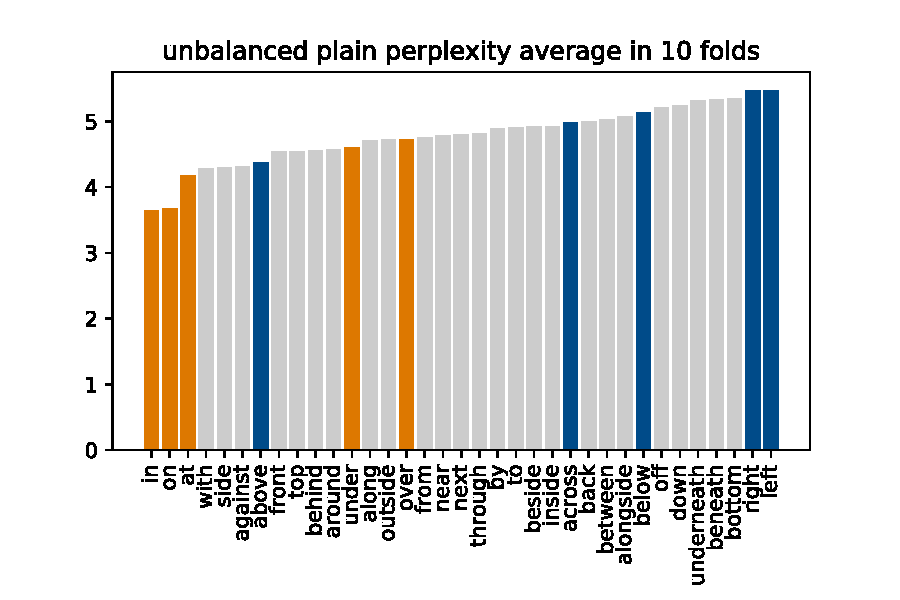
\includegraphics[width=1.12\linewidth]{studies/splu2018/figures/o_train_pp_cv-avg.pdf}\\
		(b) training set
    \end{minipage}%
  \caption{Mean perplexities of spatial descriptions of LM1 (orange:
    functionally biased, blue: geometrically biased relations).}
  \label{splu2018:fig:fig-plain-original}
\end{center}
\end{figure}


\begin{figure}[ht]
  \begin{center}
    \begin{minipage}{0.5\linewidth}
	    \centering
	    \hspace*{-1.2em}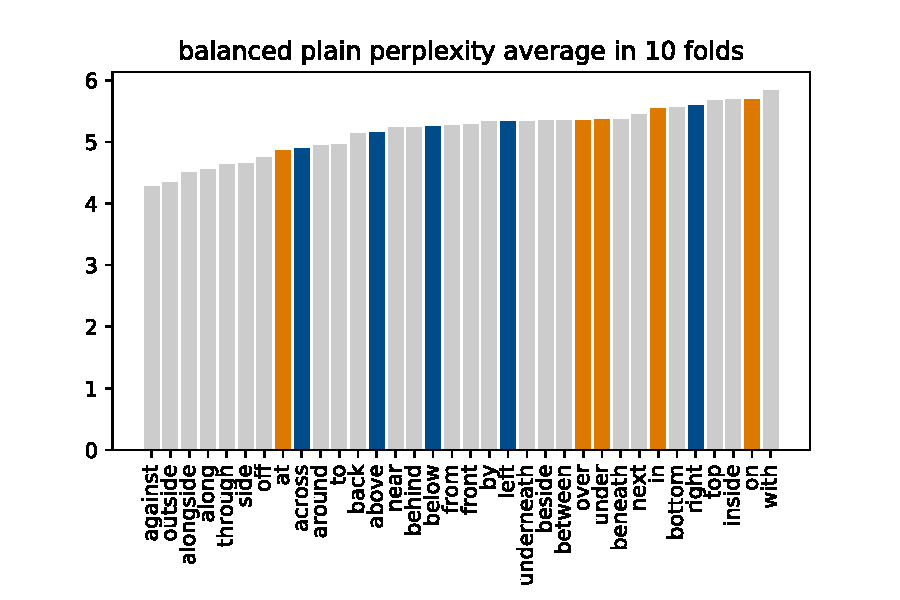
\includegraphics[width=1.12\linewidth]{studies/splu2018/figures/b_pp_cv-avg.pdf}\\
		(a) test-set 
    \end{minipage}%
    \begin{minipage}{0.5\linewidth}
	    \centering
	    \hspace*{-1.em}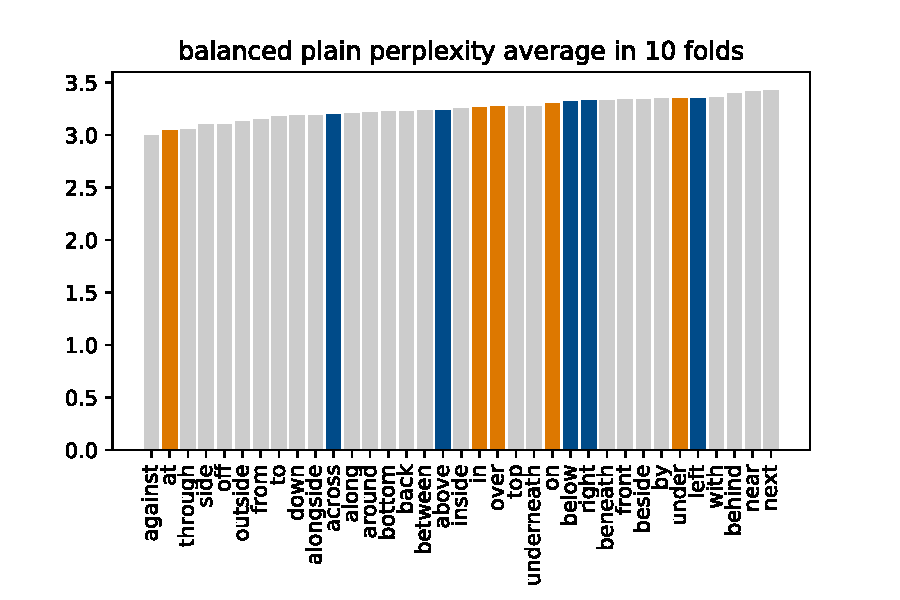
\includegraphics[width=1.12\linewidth]{studies/splu2018/figures/b_train_pp_cv-avg.pdf}\\
	    (b) training set
     \end{minipage}%
  \caption{Mean perplexities of LM2 by spatial relation (orange:
    functionally biased, blue: geometrically biased).}\label{splu2018:fig:fig-plain-balanced}
\end{center}
\end{figure}

Figure~\ref{splu2018:fig:fig-plain-original} shows the estimated average
perplexities of a subset of spatial relations, those that satisfy the sampling frequency requirement described in Section~\ref{splu2018:sec:plain-perplexity-method}. Functionally and geometrically
biased spatial relations as identified experimentally in
the literature (Section~\ref{splu2018:sec:spatial-descriptions}) are
represented with orange and blue bars respectively. There is a tendency
that functionally biased relations lead to lower mean perplexity of
phrases (Hypothesis 2 is confirmed) and also that there is a tendency that spatial
relations of a particular bias cluster together (Hypothesis 1 is also confirmed). We report results both on the training set and the test set which show the same tendencies. This means that our model generalises well on the test set and that the latter is representative.











However, in the language model the perplexities are biased by the
frequency of individual words: more frequent words are more likely and
therefore they are
associated with lower LM perplexity. %
The results show high Spearman's rank correlation coefficient $\rho=0.90$ between frequencies of spatial relation in the dataset and the perplexity of the model on the test set:
on (329,529)
$>$ in (108,880)
$>$ under (11,631)
$>$ above (8,952)
$>$ over (5,714)
$>$ at (4,890)
$>$ below (2,290)
$>$ across	(1,230)
$>$ left (996)
$>$ right (891). For the purposes of our investigation in predictability of target-landmark pairs (Hypothesis 3) we should avoid the bias in the training set.
In order to exclude the
bias of frequencies of relations, we evaluate LM2 where spatial relations are presented with equal frequencies in training. %
Figure~\ref{splu2018:fig:fig-plain-balanced} shows the ranking of spatial
relations by the perplexities when the language model was trained with
balanced frequencies. The two kinds of spatial relations are less clearly separable as the colours overlap (Hypothesis 3 is not confirmed). In comparison to Figure~\ref{splu2018:fig:fig-plain-original} there is an observable trend that all instances
lead to lower perplexities in the training set which is the effect of down-sampling on vocabulary size. Figure~\ref{splu2018:fig:fig-plain-balanced} also shows that phrases with geometrically biased spatial relations have a higher change towards lower perplexities.


Noting that the frequency of using functionally-biased spatial relations are higher in English, this bias and our strong hypothesis for predictability of target-landmark pairs can be expressed with simple joint probabilities which we are estimating with the language model:
\begin{align*}
  P(\mathrm{target, relation, landmark}) = P(\mathrm{relation}) P(\mathrm{target, landmark | relation})
\end{align*}
It is possible that targets and landmarks that occur with
these relations are very specific to these relations but
infrequent with other relations. When we remove their frequency
support provided by the frequency of relations
these targets and landmarks become infrequent in the dataset and
therefore less probable which on overall results in higher
perplexities of phrases with functionally-biased relations. Specificity of targets and landmarks can be a source of these results.


\begin{figure*}[htbp]
	\centering
  \begin{minipage}{.5\linewidth}
    \centering
    \hspace*{-1.2em}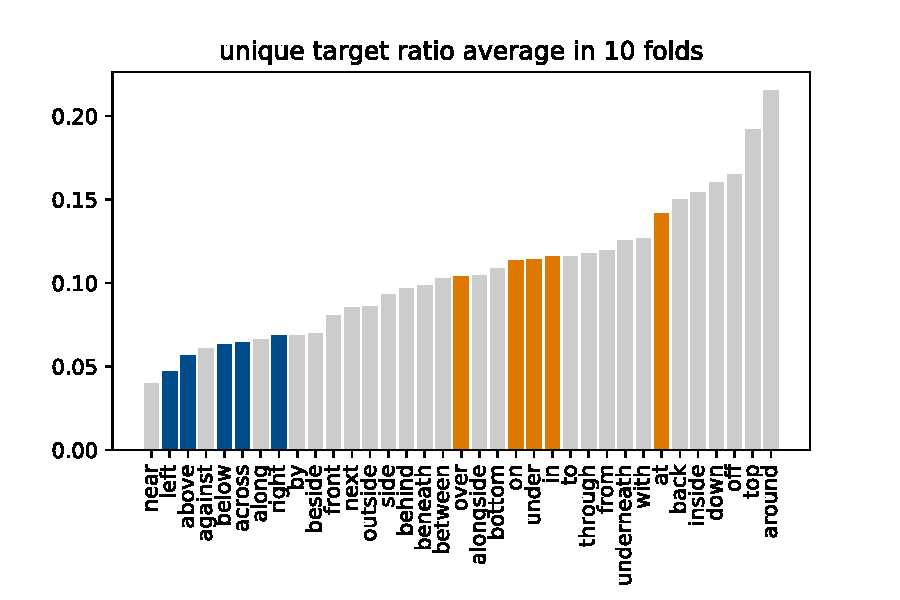
\includegraphics[width=1.12\columnwidth]{studies/splu2018/figures/train_unique_ratio-targets-avg.pdf} \\
    (a) targets
  \end{minipage}%
  \begin{minipage}{.5\linewidth}
    \centering
    \hspace*{-1.em}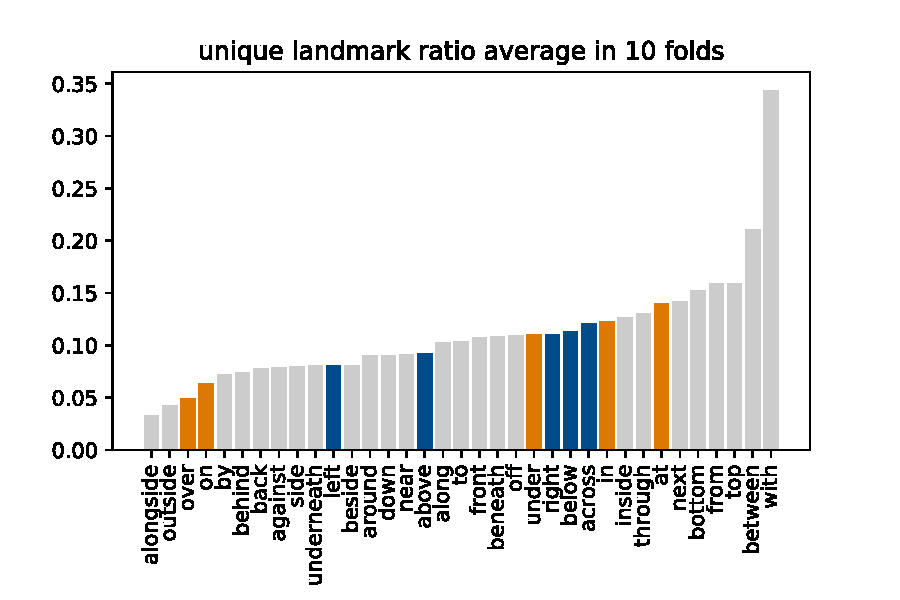
\includegraphics[width=1.12\columnwidth]{studies/splu2018/figures/train_unique_ratio-landmarks-avg.pdf} \\
    (b) landmarks
  \end{minipage}%
  \caption{Ratio between unique types and all types per spatial relation in the balanced dataset for LM2.}\label{splu2018:fig:unique-in-plain-balanced}
\end{figure*}


To provide
(some) evidence for this assumption,
Figure~\ref{splu2018:fig:unique-in-plain-balanced} shows the average ratios of
unique types over total types of targets and landmarks in the balanced
dataset over 10-folds on which LM2 was trained. There is a very clear
division between functionally and geometrically biased spatial
relations in terms of the uniqueness of targets, functionally-biased
relations are occurring with more unique ones which contributes to
higher perplexity of LM2. There is less clear distinction between the
two kinds of spatial relations in terms of uniqueness of
landmarks. Some functional relations such as \emph{on} occur with fewer
unique landmarks than targets (from .11 to .06), some geometric
relations such as \emph{right} occur with more unique landmarks than
targets (from .07 to .11). The asymmetry between targets and landmarks
is expected since the choice of landmarks in the image description
task is restricted by the choice of the targets (as well as other
contextual factors such as visual salience). They have to be ``good
landmarks'' to relate the targets to. A functional relation-landmark
pair is more related to the target through the landmark's affordances
whereas a geometric relation-landmark pair is more related to the
target through geometry. This might explain for example, why \emph{on}
has fewer, but \emph{right} has more unique landmarks than targets. On
the other hand there are also relations where the ratio of unique
targets and landmarks is very similar, for example \emph{at} (.14 and
.14). Overall, it appears that if uniqueness of objects is
contributing to the perplexity of the language model of phrases which
functionally-biased relations (which in this balanced dataset is the
case) then this is more contributed by targets rather than the
landmarks.

To further explore the idea of asymmetry between targets and landmarks
we re-arranged the targets and landmarks in the descriptions from the
balanced dataset that LM2 was trained to \texttt{$<$s$>$ landmark
  relation target $<$/s$>$} and trained LM2$'$. The average
perplexities over 10-folds of cross-validation are shown in
Figure~\ref{splu2018:fig:b_pp_cv-reversed-avg}. Comparing
Figure~\ref{splu2018:fig:b_pp_cv-reversed-avg} with
Figure~\ref{splu2018:fig:fig-plain-balanced} we first observe that the
perplexity of LM2$'$ on the descriptions is overall several magnitudes
lower than the perplexity of LM2 (max 0.06, max 140). Secondly, we
observe that the perplexities of phrases containing different
relations are very similar and that there is no separation of phrases
by perplexity depending on the relation bias. The results are in line
with our argument above. Knowing the landmark, it is much easier for
the language model to predict the relation (of either kinds) and the
target.


\begin{figure}[htbp]
  \begin{center}
  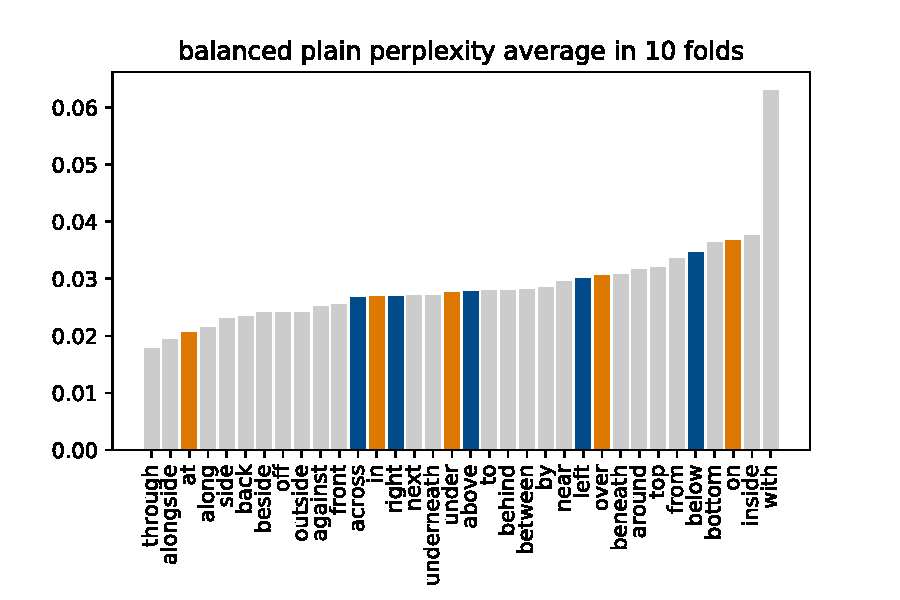
\includegraphics[width=0.6\linewidth]{studies/splu2018/figures/b_pp_cv-reversed-avg.pdf}
  \caption{Mean perplexities of LM2$'$ by spatial relation (orange: functionally biased, blue: geometrically biased)}\label{splu2018:fig:b_pp_cv-reversed-avg}
\end{center}
\end{figure}


In conclusion, the explanation why descriptions with
functionally-biased relations have a higher perplexity than
descriptions with geometrically-biased descriptions appears to be
twofold: (i) functionally-biased relations are more selective of their
targets as expressed by the uniqueness counts, and (ii) functional
relations are also more selective of their landmarks but this fact
works against the performance of the language model. As it is trained
on the sequence left to right, it has to learn to predict relations
only on the basis of targets which in the case of functionally-biased
relations are represented by more unique tokens than
geometrically-biased relations. The more informative words, the
landmarks, that would enable the language model to predict a
functional relation, comes last, after the relation has already been
seen. The possible reason why geometrically-biased relations lead to
lower perplexities of a language model on descriptions is because they
have fewer unique targets. Hence, our Hypothesis 1 which linked
selectivity of functionally-biased relations to low perplexity of
phrases can be refuted. In spatial relations the order of the semantic
interpretation of tokens (that we want to capture in these
experiments) is different from the linear syntactic order of order
which can be captured by the language model. When this order is
changed as in LM2$'$ our predictions come closer to the hypothesis
(Figure~\ref{splu2018:fig:b_pp_cv-reversed-avg}).\footnote{Modulo that
  landmarks are, as discussed above, well-predictive of relations of
  both kinds.} %







By removing the frequency bias on spatial relations in LM2 we fix the
distribution of spatial relations and examine the effect of
distribution of targets and landmarks on perplexities of phrases
(spatial relation as fixed context). In the following section, we fix
the distributions of targets and landmarks of each spatial relation
and examine the perplexity of phrases when another spatial relation is
projected in this context (targets-landmarks as fixed context).





\section{Varying spatial relations}\label{splu2018:sec:swapability}



\subsection{Hypotheses}

Given a particular spatial relation, the distribution of targets and
landmarks that occur with it creates a particular signature of targets
and landmarks, the target-landmark context of a spatial relation. In
this experiment, we investigate the effect on perplexity of phrases
when another spatial relation is projected in such a target-landmark
context. Given different selectivity of functionally- and
geometrically-biased spatial relations, namely the functionally-based
spatial relations are more selective of their targets and landmarks
and therefore create more specific contexts, we should observe
differences in perplexities of phrases when other spatial relations
are projected in these contexts. In particular, we hypothesise that
geometrically-biased spatial relations are more easily swappable than
functionally-biased spatial relations as measured by the perplexity of
a language model trained on the original, non-swapped phrases
(Hypothesis 4).











\subsection{Method}

We use %
LM2 from Section~\ref{splu2018:sec:plain-perplexity} (trained on the balanced
frequencies of spatial relations) with no additional training from the
previous experiment. We group descriptions in the evaluation set by
spatial relation. For each phrase containing a particular spatial
relation, we replace it with every other spatial relation and estimate
the perplexity of the resulting phrase using a language
model. Finally, we calculate the mean of perplexities over all
phrases. We use 10-fold cross-validation and report the final means
across the 10 folds.






\subsection{Results}











\begin{figure}[htbp]
  \begin{center}
  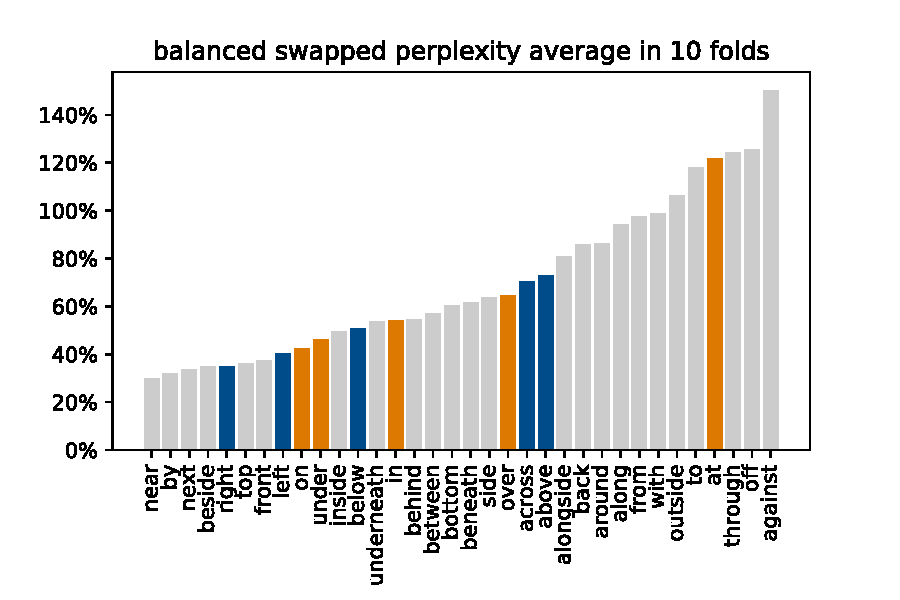
\includegraphics[width=0.6\linewidth]{studies/splu2018/figures/b_swapped_cv-avg.pdf}
  \caption{\%-increase in perplexities of LM2 shown per context of the original preposition when swapped with another one.}
  \label{splu2018:fig:fig-swap-balanced}
\end{center}
\end{figure}


Figure~\ref{splu2018:fig:fig-swap-balanced} shows a \%-increase in mean
complexities from those in Figure~\ref{splu2018:fig:fig-plain-balanced} when
LM2 is applied on phrases with swapped relations in the contexts of
the original relations. Hence, the column ``at'' shows the \%-increase
in perplexities of phrases that originally contained \emph{at} in the
validation dataset but this was replaced by all other spatial
relations. Comparing with Figure~\ref{splu2018:fig:fig-plain-balanced} the
estimated perplexities are higher across all cases which is
predictable. There is a weak tendency that replacing
functionally-biased relations with other relations leads to higher
perplexities of spatial descriptions than replacing
geometrically-biased relations, but the distinction is not
clear cut (Hypothesis 4 partially confirmed). The lack of a clear
distinction between two classes of descriptions confirms our previous
observations about landmarks and targets: the LM has learned
particular contexts for both kinds of descriptions.


















\section{Discussion and conclusion}
\label{splu2018:sec:discussion}


We explored the degree that the functional and geometric character of
spatial relations can be identified by a neural language model by
focusing on spatial descriptions of controlled length and containing
normalised relations. Our first question was about the implications of
using a neural language model for this task. The previous research
\cite{Dobnik:2013aa} used normalised entropy of target-landmarks per
relation and log likelihood ratio between target-landmarks and
relations to test this. These are focused measures that estimate the
variation and the strength of association of words in a corpus. On the
other hand, a language model provides a more general probabilistic
representation of the entire description. As such it captures any kind
of associations between words in a sequence. The other important
observation is that it captures sequential relations in the direction
left to right and as we have seen the sequential nature of the
language model does not correspond precisely with the order in which
semantic arguments of spatial relations are interpreted. However,
nonetheless we can say that language models are able to capture a
distinction between functional and geometric spatial relations (plus
other semantic distinctions) to a similar degree of success as
previously reported measures. Our initial hypothesis about the greater
selectivity of spatial relations for its arguments is correct but it
is exemplified in a greater perplexity of a language model in the
context of balanced spatial relations. We argued that this has to do
with the fact that the targets are more unique to these relations
(which is consequence of a greater specificity for arguments of
functionally biased relations) and is also related to the way a
sequential language model works. In the unbalanced dataset, the
perplexity of the language model is reversed (it is lower with
functionally biased relations) because the specificity of targets to
relations is boosted with greater frequency of functionally-biased
relations. The fact that functionally-biased relations are more
frequent is probably related to the fact that such descriptions are
more informative than purely geometric ones if available for a
particular pair of objects.

We can only report tendencies based on the perplexities of our
language models as our conclusions. This is because the
functional-geometric bias is graded, because the predictions are
highly dependent on the quality and the size of the dataset, and
because other semantic relations might also be expressed by this
measure. We chose a large contemporary dataset of image descriptions
because we hope that it contains a high proportion of prepositions
used as spatial relations. However, there is no guarantee that all
prepositions in this dataset are used this way. We observe that there
is considerable variation of obtained values across the 10-folds of
cross-validation %
and we report the mean values over all folds. As an illustration, in
the supplementary material (Section~\ref{splu2018:sec:evaluation-variation}) we
give an example of graphs from two intermediary folds.


Using a language model in this task we have also learned new insights
about the way language models encode spatial relations in image
descriptions. It has been pointed out (cf. \cite{kelleher2017what}
among others) that convolutional neural networks with an attention
model are designed to detect objects whereas spatial relations between
objects are likely to be predicted by the language model. In this work
we show that language models are not only predicting the relation
(which is expected) but are able to distinguish between different
classes of relations thus encoding finer semantic distinctions. This
tells us that language models are able to encode a surprising amount
of information about world knowledge with a usual caveat that it is
difficult to separate several strands of this knowledge.

The work can be extended in several ways. One way is to study dataset
effects on the predicted results. Datasets with descriptions of
robotic actions and instructions may be particularly promising as they
focus on spatial uses. Different normalisations of spatial relations
have a significant effect on the results. In this work composite
spatial relations such \emph{on the left side of} are normalised to
simple spatial relations such as \emph{left}. However, these could be
treated as separate relations as difference between may exist. A more
systematic examination of clusters of spatial relations would
eventually tell us what other spatial relations not yet identified as
functionally or geometrically biased have similar properties to those
that have identified as such experimentally.






\section*{Acknowledgements}

The research of Dobnik and Ghanimifard was supported by a grant from the Swedish Research Council (VR project 2014-39) for the establishment of the Centre for Linguistic Theory and Studies in Probability (CLASP) at Department of Philosophy, Linguistics and Theory of Science (FLoV), University of Gothenburg.

The research of Kelleher was supported by the ADAPT Research Centre. The ADAPT Centre for Digital Content Technology is funded under the SFI Research Centres Programme (Grant 13/RC/2106) and is co-funded under the European Regional Development Funds.


\section{Appendix: Supplementary material}

\subsection*{Language Model Architecture}\label{splu2018:sec:lm}

\begin{figure}[ht!]
  \begin{center}
  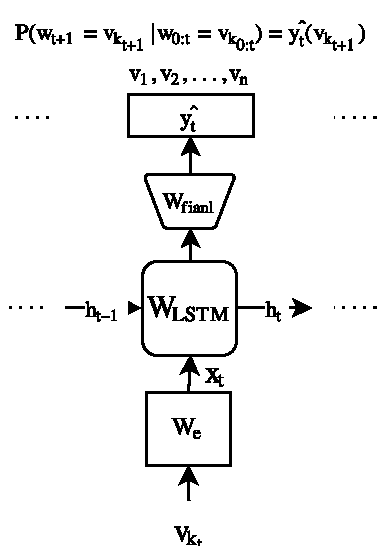
\includegraphics[width=0.35\linewidth]{studies/splu2018/figures/lm_diagram.pdf} \\
  \caption{The recurrent language model diagram with LSTM recurrent unit.}
  \label{splu2018:fig:lm-diagram}
  \end{center}
\end{figure}

The neural language model architecture with the Long-Short Terms Memory (LSTM) function and its parameters, similar to tied weights in \cite{gal2016theoretically}:
\begin{itemize}[topsep=0em,itemsep=0em,partopsep=0em,parsep=0em]
  \item $W_e \in {R}^{n \times d}$ for word embeddings,
  \item $W_{LSTM} \in {R}^{2d \times 4d}$ for parameters of the Long-Short Term
  Memory function,
  \item $W_{Final} \in {R}^{d \times n}$ of the final dense layer with
  \emph{softmax}.
\end{itemize}
\noindent where $n$ is the vocabulary size for $V = \{ v_1, v_2, ..., v_{n} \}$ and $d$
is both the embeddings size and the memory size in LSTM.
For mini-batches from training data, these parameters are being updated using a
stochastic gradient descent to minimise the loss.
\begin{align}\label{splu2018:eq:lm-parameters}
x_{t} &= \delta_{v_{k_t}} \cdot W_e \\
\begin{pmatrix}
\text{i} \\
\text{f} \\
\text{o} \\
\text{g}
\end{pmatrix}
& =
\begin{pmatrix}
\sigma \\
\sigma \\
\sigma \\
\text{tanh}
\end{pmatrix}
\bigg(
\begin{pmatrix}
\text{x}_t \\
\text{h}_{t-1}
\end{pmatrix}
\cdot
\text{W}_{LSTM}
\bigg) \\
c_t & = \text{f} \circ c_{t-1} + \text{i} \circ \text{g} \\
h_t & = \text{o} \circ \text{tanh}(c_t) \\
\hat{y}_t & = \text{softmax}(h_t \cdot \text{W}_{final} + b)
\end{align}
\noindent where $\delta_{v_{k_t}}$ represents the one-hot encoding of the $t$-th word in
the sequence. The $x_{t}$ is the word embedding for this word, and two vectors $c_t$ and $h_t$ represent the states of the recurrent unit. Figure~\ref{splu2018:fig:lm-diagram} illustrates the same equation.

\subsection*{Evaluation}\label{splu2018:sec:evaluation-variation}

\begin{figure}[ht!]
  \centering
  \begin{minipage}{.5\textwidth}
    \centering
    \hspace*{-1.2em}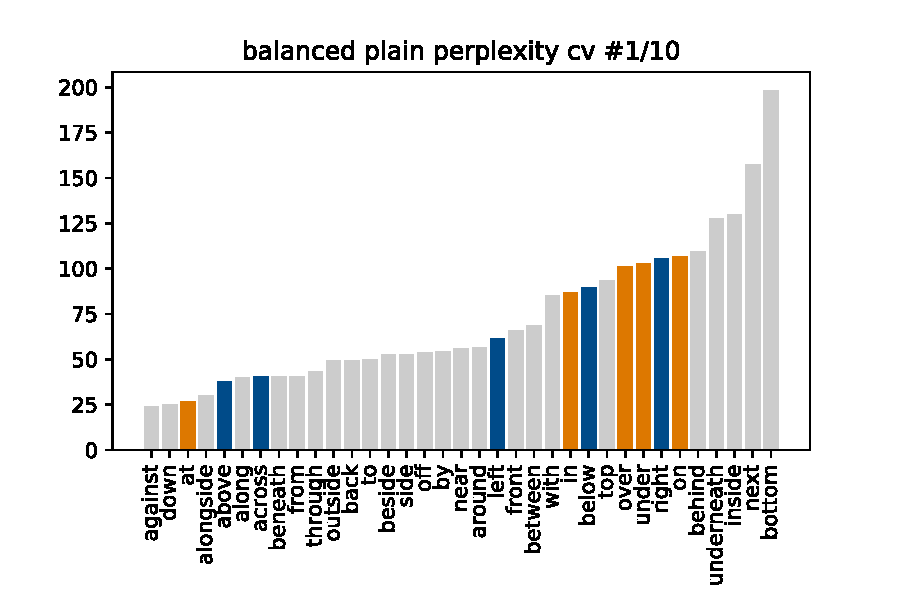
\includegraphics[width=1.12\columnwidth]{studies/splu2018/figures/b_pp_cv-f1.pdf} \\
    (a)
  \end{minipage}%
  \begin{minipage}{.5\textwidth}
    \centering
    \hspace*{-1.em}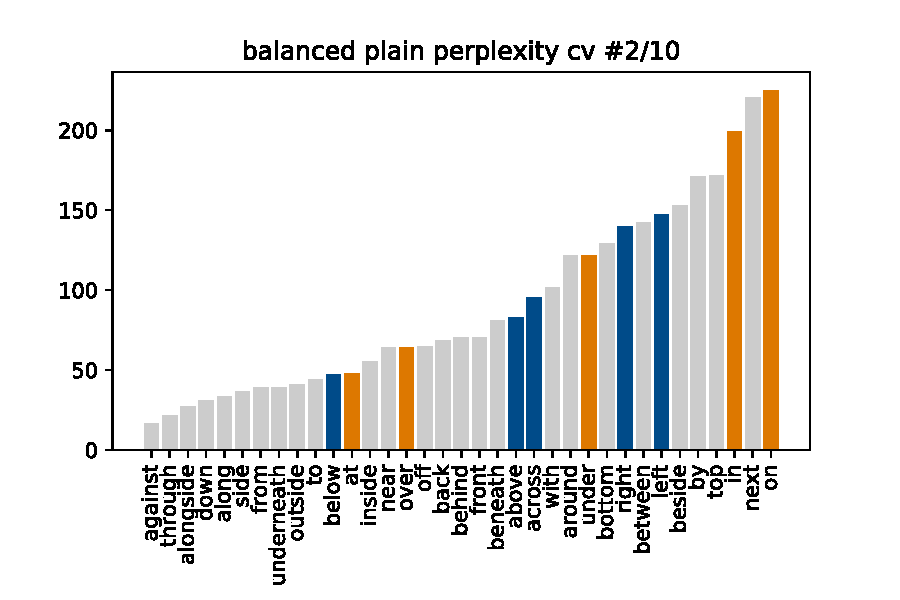
\includegraphics[width=1.12\columnwidth]{studies/splu2018/figures/b_pp_cv-f2.pdf} \\
    (b)
  \end{minipage}
  \caption{Mean perplexities of LM2 by spatial relation for (a) folds 1 and (b) 2 (orange:
    functionally biased, blue: geometrically biased).}\label{splu2018:fig:fig-plain-balanced-folds}
\end{figure}


\clearpage
\bibliographystyle{acl_natbib}
\bibliography{studies/splu2018/references.bib}
